\chapter{Розділ 1: Основні класи множин}
\phantomsection
\addcontentsline{toc}{chapter}{Основні класи множин}

%Нехай $X$ є фіксованою непорожньою множиною, яку називатимемо універсальною. Через $2^X$ позначимо множину усіх підмножин $X$ (включаючи порожню множину і саму множину $X$).
%
%
%\section{Означення основних класів множин}
%
%\begin{definition}
%	\label{def-1-1}
%	Непорожній клас $\HH\subset 2^X$ називається \emph{кільцем}, якщо
%	\begin{enumerate}[label={\upshape (\roman*)}]
%		\item \label{def-1-1-i}
%		$\forall A\in\HH\ \forall B\in\HH\quad A\cup B\in\HH $;
%		\item \label{def-1-1-ii}
%		$\forall A\in\HH\ \forall B\in\HH\quad A\setminus B\in\HH $.
%	\end{enumerate}
%\end{definition}
%
%\begin{definition}
%	\label{def-1-2}
%	Непорожній клас $\HH\subset 2^X$ називається \emph{алгеброю}, якщо
%	\begin{enumerate}[label={\upshape (\roman*)}]
%		\item \label{def-1-2-i}
%		$\HH $ є кільцем;
%		\item \label{def-1-2-ii}
%		$X\in\HH $.
%	\end{enumerate}
%\end{definition}
%
%\begin{example}
%	\label{ex-1-1}
%	$\HH=2^X$ є алгеброю.
%\end{example}
%
%\begin{example}
%	\label{ex-1-2}
%	Нехай $X$ є довільною нескінченною множиною. Тоді клас усіх її скінченних підмножин є кільцем.
%\end{example}
%
%\begin{example}
%	\label{ex-1-3}
%	Нехай $X$ є довільною нескінченною множиною. Тоді клас усіх її скінченних підмножин  та їх доповнень  є алгеброю.
%\end{example}
%
%Наступне твердження дає нам деякі \emph{властивості кілець}.
%
%\begin{statement}
%	\label{st-pr-ring}
%	Нехай $\K$ є кільцем. Тоді
%	\begin{enumerate}
%		\item \label{st-pr-ring-1}
%		$\emptyset\in\K$;
%		\item \label{st-pr-ring-2}
%		$\forall A\in\HH\ \forall B\in\HH\quad A\cap B\in\HH $;
%		\item \label{st-pr-ring-3}
%		$\forall \{A_k\}_{k=1}^n\subset\K \quad
%		\displaystyle \left(\bigcup_{k=1}^n A_k\in\K \  \land \  \bigcap_{k=1}^n A_k\in\K\right)$.
%	\end{enumerate}
%\end{statement}
%
%\begin{proof}
%	\ref{st-pr-ring-1}.
%	Оскільки $\K\neq\emptyset$, то знайдеться  $A\in\K$, отже, $\emptyset=A\setminus A\in\K$ за умовою \ref{def-1-1-ii} означення \ref{def-1-1}.
%
%	\ref{st-pr-ring-2}.
%	Маємо $A\cap B=A\setminus(A\setminus B)$. За умовою \ref{def-1-1-ii} означення \ref{def-1-1} різниця елементів кільця належить кільцю (див. рис.~\ref{fig-1-1}).
%
%	\ref{st-pr-ring-3} одразу випливає з умови \ref{def-1-1-i} означення \ref{def-1-1} і щойно доведеної властивості \ref{st-pr-ring-2}.
%\end{proof}
%
%\begin{figure}[!h]
%	\centering
%	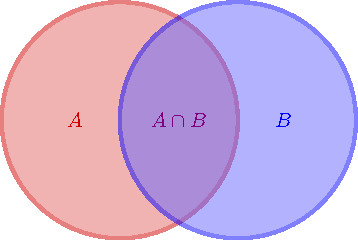
\includegraphics{fig-1-1}
%	\caption{Подання $A\cap B$.}
%	\label{fig-1-1}
%\end{figure}
%
%\begin{definition}
%	\label{def-1-3}
%	Непорожній клас $\HH\subset 2^X$ називається \emph{півкільцем}, якщо
%	\begin{enumerate}[label={\upshape (\roman*)}]
%		\item \label{def-1-3-i}
%		$\forall A\in\HH\ \forall B\in\HH\quad A\cap B\in\HH $;
%		\item \label{def-1-3-ii}
%		$\forall A\in\HH \forall B\in\HH\ \exists \{C_k\}_{k=1}^n\subset\HH\quad
%		\displaystyle \bigg(A\setminus B= \bigcup_{k=1}^n C_k\  \land \ \{C_k\}_{k=1}^n$ є неперетинними\bigg).
%	\end{enumerate}
%\end{definition}
%
%Ми називаємо множини $\{C_k\}_{k=1}^n\subset X$ \emph{неперетинними}, якщо
%$$
%\forall k=\overline{1,n}\ \forall p=\overline{1,n}\quad \big(k\neq p \Rightarrow C_k\cap C_p=\emptyset\big).
%$$
%
%\begin{definition}
%	\label{def-1-3-a}
%	Непорожній клас $\HH\subset 2^X$ називається \emph{півалгеброю}, якщо
%	\begin{enumerate}[label={\upshape (\roman*)}]
%		\item \label{def-1-3-a-i}
%		$\HH $ є півкільцем;
%		\item \label{def-1-3-a-ii}
%		$X\in\HH $.
%	\end{enumerate}
%\end{definition}
%
%Зазначимо, що якщо $\PP\subset 2^X$ є півкільцем, то $\emptyset\in\PP$. \label{semi-ring-emptyset} Дійсно, для довільної множини $A\in\PP$ існують неперетинні множини  $\{C_k\}_{k=1}^n\subset\PP$, дя яких
%$$
%\emptyset=A\setminus A= \bigcup_{k=1}^n C_k,
%$$
%що можливо лише для $C_k=\emptyset$, $k=\overline{1,n}$.
%
%\begin{example}
%	\label{ex-1-4}
%	Нехай
%	$$
%	\PP_1=\{(a,b]\mid a\in\R \land b\in\R\}.
%	$$
%	Зрозуміло, що $\PP_1$ є півкільцем для $X=\R$.
%\end{example}
%
%\begin{remark}
%	Для інтервалу $(a,b]$ завжди вважатимемо, що $a\leq b$ і $(a,a]=\emptyset$.
%\end{remark}
%
%Розглянемо \emph{теорему про добуток кілець}.
%
%\begin{theorem}
%	\label{th-1-1}
%	Нехай $X_1$, $X_2$, \ldots, $X_d$ є основними множинами і $\HH_1\subset 2^{X_1}$, $\HH_2\subset 2^{X_2}$, \ldots,  $\HH_d\subset 2^{X_d}$ є півкільцями. Тоді клас множин
%	\begin{align*}
%	\HH&=\HH_1\times\HH_2\times\cdots\times\HH_d
%	\\
%	&=\{A_1\times A_2\times\cdots\times A_d\mid A_1\in\HH_1 \land A_2\in\HH_2 \land \cdots \land A_d\in\HH_d\}
%	\end{align*}
%	є півкільцем підмножин множини $X=X_1\times X_2 \times\cdots\times X_d$.
%\end{theorem}
%
%\begin{proof}
%	Перевіримо виконання умов означення \ref{def-1-3} для $d=2$. Клас $\HH$ є непорожнім, оскільки непорожніми є класи $\HH_1$ і $\HH_2$.
%
%
%	Нехай $A\in\HH$ і $B\in\HH$. Тоді $A=A_1\times A_2$ і $B=B_1\times B_2$, де $A_1\in\HH_1$, $A_2\in\HH_2$, $B_1\in\HH_1$, $B_2\in\HH_2$.
%
%	\ref{def-1-3-i}
%	Оскільки $\HH_1$ і $\HH_2$ є півкільцями, то за означенням \ref{def-1-3} маємо
%	$$
%	A_1\cap B_1\in\HH_1, \quad A_2\cap B_2\in\HH_2.
%	$$
%	Маємо (див. рис.~\ref{fig-1-2})
%	$$
%	A\cap B= (A_1\cap B_1)\times (A_2\cap B_2),
%	$$
%	отже, $A\cap B\in\HH$.
%
%\begin{figure}[!h]
%	\centering
%	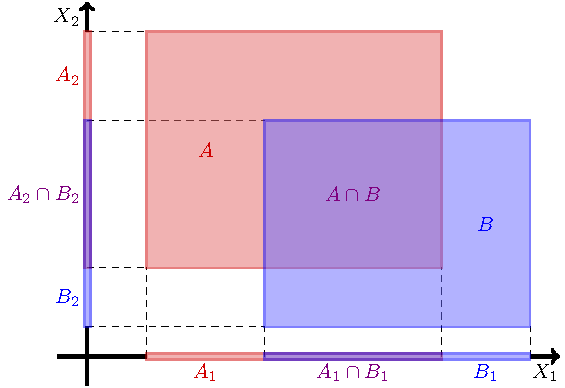
\includegraphics{fig-1-2}
%	\caption{Подання $A\cap B$.}
%	\label{fig-1-2}
%\end{figure}
%
%	\ref{def-1-3-ii}
%	Оскільки $\HH_1$ і $\HH_2$ є півкільцями, то за означенням \ref{def-1-3}
%	$$
%	A_1\setminus B_1=\bigcup_{k=1}^n C_k, \quad A_2\setminus B_2=\bigcup_{i=1}^j D_i,
%	$$
%	де $\{C_k\}_{k=1}^n\subset \HH_1$ і $\{D_i\}_{i=1}^j\subset \HH_2$ є неперетинними. Оскільки (див. рис.~\ref{fig-1-3})
%	$$
%	A\setminus B = (A_1\times A_2)\setminus(B_1\times B_2) = \big((A_1\setminus B_1)\times A_2\big)\cup \big((A_1\cap B_1)\times (A_2\setminus B_2)\big),
%	$$
%	то
%	$$
%	A\setminus B = \left(\bigcup_{k=1}^n (C_k\times A_2) \right) \cup \left(\bigcup_{i=1}^j \big((A_1\cap B_1)\times D_i\big) \right)
%	$$
%\begin{figure}[!h]
%	\centering
%	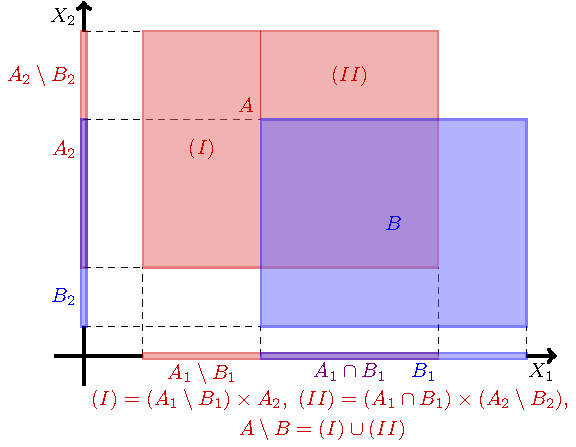
\includegraphics{fig-1-3}
%	\caption{Подання $A\setminus B$.}
%	\label{fig-1-3}
%\end{figure}
%	Усі декартові добутки у правій частині цієї рівності належать $\HH$ і є неперетинними, оскільки множини $\{C_k\}_{k=1}^n\subset \HH_1$ і $\{D_i\}_{i=1}^j\subset \HH_2$ є неперетинними.
%
%	Таким чином, ми перевірили виконання умов \ref{def-1-3-i} і \ref{def-1-3-ii} означення 	\ref{def-1-3} для $d=2$. Звідси одразу випливає і загальний випадок для довільного $d$. Теорему доведено.
%\end{proof}
%
%\begin{example}
%	\label{ex-1-5}
%	Нехай
%	$$
%	\PP_d=\left\{\bigtimes_{k=1}^d(a_k,b_k] \midd \forall k=\overline{1,d}\quad a_k\in\R \land b_k\in\R\right\}.
%	$$
%	Клас $\PP_d$ є півкільцем підмножин множини $X=\R^d$ за теоремою \ref{th-1-1} про добуток кілець, оскільки $\PP_d=\PP_1\times\PP_1\times \cdots \times \PP_1$ (див. приклад \ref{ex-1-1}).
%\end{example}
%
%Розглянуті класи множин пов'язані зі скінченними об'єднаннями і перетинами множин. Далі нам знадобляться ще й класи множин, пов'язані зі зліченними об'єднаннями і перетинами.
%
%\begin{definition}
%	\label{def-1-4}
%	Непорожній клас $\HH\subset 2^X$ називається \emph{$\sigma$-кільцем}, якщо
%	\begin{enumerate}[label={\upshape (\roman*)}]
%		\item \label{def-1-4-i}
%		$\forall \{A_n\}_{n=1}^\infty\subset\HH\quad
%		\displaystyle  \bigcup_{n=1}^\infty A_k\in\HH $;
%		\item \label{def-1-4-ii}
%		$\forall A\in\HH\ \forall B\in\HH\quad A\setminus B\in\HH $.
%	\end{enumerate}
%\end{definition}
%
%\begin{example}
%	\label{ex-1-6}
%	Нехай $X$ є довільною нескінченною множиною. Тоді клас усіх її скінченних і зліченних підмножин  є  $\sigma$-кільцем.
%\end{example}
%
%\begin{definition}
%	\label{def-1-5}
%	Непорожній клас $\HH\subset 2^X$  називається \emph{$\sigma$-ал\-геб\-рою}, якщо
%	\begin{enumerate}[label={\upshape (\roman*)}]
%		\item \label{def-1-5-i}
%		$\HH $ є $\sigma$-кільцем;
%		\item \label{def-1-5-ii}
%		$X\in\HH $.
%	\end{enumerate}
%\end{definition}
%
%\begin{example}
%	\label{ex-1-7}
%	Нехай $X$ є довільною нескінченною множиною. Тоді клас усіх її скінченних і зліченних підмножин  та їх доповнень є  $\sigma$-алгеброю.
%\end{example}
%
%\begin{example}
%	\label{ex-1-8}
%	Нехай $X$ є довільною  множиною. Тоді клас $\HH=\{\emptyset, X\}$ є  $\sigma$-алгеброю (її називають тривіальною).
%\end{example}
%
%Наступне твердження дає нам деякі \emph{властивості $\sigma$-кілець}.
%
%\begin{statement}
%	\label{st-pr-sring}
%	Нехай $\SSS$ є $\sigma$-кільцем. Тоді
%	\begin{enumerate}
%		\item \label{st-pr-sring-1}
%		$\SSS$ є кільцем;
%		\item \label{st-pr-sring-2}
%		$\forall \{A_n\}_{n=1}^\infty\subset\SSS \quad
%		\displaystyle  \bigcap_{n=1}^\infty A_n\in\SSS$.
%	\end{enumerate}
%\end{statement}
%
%\begin{proof}
%	Для доведення властивості \ref{st-pr-sring-1} маємо перевірити умову \ref{def-1-1-i} означення \ref{def-1-1}. Для $A\in\SSS$ і $B\in\SSS$ за умовою \ref{def-1-5-i} означення \ref{def-1-5} маємо
%	$$
%	A\cup B= A\cup B\cup B\cup B\cup \cdots \in\SSS.
%	$$
%	Оскільки другі умови в означеннях \ref{def-1-1} і \ref{def-1-5} збігаються, звідси випливає, що $\SSS$ є кільцем.
%
%	Властивість \ref{st-pr-sring-2} випливає з умови \ref{def-1-5-ii} означення \ref{def-1-5} і подання (див. рис.~\ref{fig-1-4})
%	$$
%	\bigcap_{n=1}^\infty A_n= A_1\setminus \left( \bigcup_{n=2}^\infty (A_1\setminus A_n)\right)\in\SSS.
%	$$
%
%	Теорему доведено.
%\end{proof}
%
%\begin{figure}[!h]
%	\centering
%	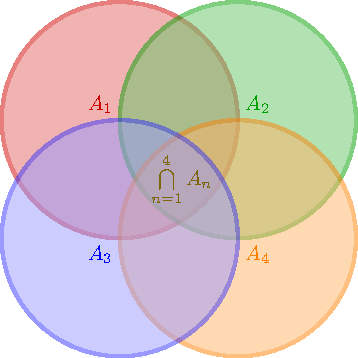
\includegraphics{fig-1-4}
%	\caption{Подання перетину множин.}
%	\label{fig-1-4}
%\end{figure}
%
%\begin{definition}
%	\label{def-incr}
%	Послідовність множин $\{A_n\}_{n=1}^\infty\subset X$
%	називається \emph{неспадною}, якщо
%	$$
%	\forall n\in\N\quad A_n\subset A_{n+1}.
%	$$
%	Це позначатимемо $\{A_n\}_{n=1}^\infty\uparrow$ і покладемо
%	\begin{equation}
%	\label{1.2}
%	\lim_{n\to\infty} A_n= \bigcup_{n=1}^\infty A_n.
%	\end{equation}
%\end{definition}
%
%\begin{definition}
%	\label{def-decr}
%	Послідовність множин $\{A_n\}_{n=1}^\infty\subset X$
%	називається \emph{незростальною}, якщо
%	$$
%	\forall n\in\N\quad A_n\supset A_{n+1}.
%	$$
%	Це позначатимемо $\{A_n\}_{n=1}^\infty\downarrow$ і покладемо
%	\begin{equation}
%	\label{1.3}
%	\lim_{n\to\infty} A_n= \bigcap_{n=1}^\infty A_n.
%	\end{equation}
%\end{definition}
%
%\begin{definition}
%	\label{def-mon}
%	Послідовність множин називається \emph{монотонною}, якщо вона є незростальною або неспадною.
%\end{definition}
%
%\begin{definition}
%	\label{def-1-6}
%	Непорожній клас $\HH\subset X$ називається \emph{монотонним класом}, якщо для будь-якої послідовності $\{A_n\}_{n=1}^\infty\subset \HH$ маємо $\displaystyle\lim_{n\to\infty} A_n\in\HH$.
%\end{definition}
%
%Розглянемо \emph{теорему про зв'язок між кільцем і монотонним класом}.
%
%\begin{theorem}
%	\label{th-1-2}
%	Нехай клас $\HH\subset 2^X$ є кільцем і монотонним класом. Тоді $\HH$ є $\sigma$-кільцем.
%\end{theorem}
%
%\begin{proof}
%	Порівнюючи означення \ref{def-1-1} (кільця) і \ref{def-1-5} ($\sigma$-кільця) бачимо, що для доведення теореми досить довести виконання умови  \ref{def-1-5-i} означення \ref{def-1-5}. Нехай $\{A_n\}_{n=1}^\infty\subset \HH$. Позначимо
%	$$
%	B_n=\bigcup_{k=1}^n A_k,\quad n\in\N.
%	$$
%	Маємо $B_n\in\HH$, $n\in\N$, тому, що $\HH$ є кільцем. За побудовою
%	$$
%	\forall n\in\N\quad B_n\subset B_{n+1}.
%	$$
%	тобто $\{B_n\}_{n=1}^\infty\uparrow$. Оскільки $\HH$ є монотонним класом, маємо
%	$$
%	\HH\ni\lim_{n\to\infty} B_n=\bigcup_{n=1}^\infty B_n= \bigcup_{n=1}^\infty A_n.
%	$$
%	Остання рівність виконується за побудовою послідовності $\{B_n\}_{n=1}^\infty$. Таким чином, теорему доведено.
%\end{proof}

